\section{Mathematical Modeling}
\label{sec:mathmodel}

% \begin{itemize}
% \item \st{unstable stratified boundary layers (raleigh number estimate)}
% \item \st{justify incompressible N-S}
% \item \st{justification of far-field eddy-viscosity model (M-O)}
% \item modeling eddy-viscosity in device 
% \item vane and turbine representation via penalty function // immersed boundary method
% \item cone representation
% \end{itemize}

%remember that \st{} is strikethrough
%
% should this all be math modeling?
%

Our aim is to simulate the formation of synthetic dust devils in the
field. This requires a model of the ambient conditions for a
representative case, such as Arizona, where experimental data is
available from test have been performed. Furthermore, for this to be
more generally useful in the prediction of flows in a variety of
conditions, we need a model generally applicable to any flow near the
surface of the earth.  

This section details an analysis of surface fluid mechanics, and
develops a mathematical model for turbulence in a thermally stratified
medium. We seek to emulate the operation of the apparatus during the day, 
when dust devils are observed to form readily. 
At these times, the atmospheric surface layer has the following character. 
Incident radiation from the sun largely does not interact with the
air, which is nearly transparent. Instead, this radiation is absorbed by
the ground, which causes a temperature rise. This results in a thermal
gradient between the hot ground and the cooler air. The warm ground
conducts heat to the air, causing an expansion and lowering the density
of the air. This reduced density air near the surface is driven upwards
by the force of buoyancy.  

For sufficiently large temperature gradients, these motions are
unstable, and as the warm air is driven upwards the flow will transition
to turbulence. For the typical use case we consider, namely Arizona in
summer, the temperature gradient can be in excess of 30 Kelvin. 
Rayleigh numbers associated with this are typically between $10^{9} -
10^{11}$, and therefore meet the criterion for transition to a turbulent
regime. The flow is that of an unstably stratified fluid. 

\subsection{Equations of Fluid Motion}
%
% do I need to justify this more? These are pretty critical, after all
%

The equations describing fluid flow at
low Mach number with natural convection are, %\todo{fix me up}
\begin{eqnarray*}
 \frac{\partial u}{\partial t} + u \cdot \nabla u =&
  -\frac{1}{\rho}\nabla P + \nu \nabla^2 u - g \frac{T'}{T_0}\\
 \nabla \cdot u =& 0 \\
 \rho c_p \frac{\partial T}{\partial t} =& \nabla \cdot ( k \nabla T).
\end{eqnarray*} 
Where we have made the assumptions that the temperature gradient is small in
comparison to the mean temperature of the region. These are the
incompressible Navier-Stokes equations for free-convection (or
``Boussinesq'') coupled with the heat equation. 
%
% in full document be sure to mention that neglecting coriolis is legit
% below 50ms
%
%
As discussed above, we anticipate our flow to be
turbulent. Turbulence significantly alters the character of the flow,
and necessitates either resolving the resulting small scales or
providing a model that emulates their impact. In this case, we use
essentially a Reynolds Averaged Navier-Stokes (RANS) model, where we
permit the viscosity and thermal conductivities to vary in space, and
decompose the flow into constant laminar and varying turbulent and vane
components,  
\begin{eqnarray*}
 \nu =& \nu_{l} + \nu_{T}(z) + \nu_{V}(r,z) \\
 K =& K_{l} + K_{T}(z) + K_{V}(r,z)
\end{eqnarray*}

This is an effective eddy viscosity model, and the subsequent two
sections will elaborate on the spatial dependence and character of
$\nu_T$, $K_T$, $\nu_C$ and $K_C$. $\nu_l$ and $K_l$ are the laminar,
base diffusivities and do not vary in space. 

\subsection{Viscosity Model}

We use the celebrated similarity model of Monin and
Yaglom\cite{monin2007statistical,monin1954basic} as a guide to the
present development, which we outline below. Their work is extension of
the mixing-length model of Prandtl, where the concepts of gradient
diffusion and mixing length were generalized to thermally stratified
flow.   

%
% justify prandtl assumption here
%

We begin by using dimensional analysis, and noting that the dynamics of
any mean quantity ($\bar f$) in a thermally stratified medium only depend on,

\begin{equation}
\bar f = f(z_0,\frac{g}{T_0},\rho_0,\nu_l,K_l,u^*,q)
\end{equation}

We expect that aside from very near the surface, the diffusivities $\nu_l$
and $K_l$ will be small compared to their turbulent counter-parts, $\nu_T$
and $K_T$. Likewise, if we define $z-z_0$ as an ``effective roughness
height'' or displacement distance, we can reasonably neglect $z_0$ from these
considerations. While the roughness height can be large (for instance in
a cornfield, where the roughness height could reasonably be several
meters), for our present study the expectation is that this roughness
height will be on the order of centimeters\cite{oke1987boundary}, and
therefore negligible.  

This leaves only five parameters: the distance from the ground, z; the
buoyancy coefficient, $\frac{g}{T_0}$; the density of the fluid,
$\rho_0$; a velocity scale, $u^*$; and the heat flux from the ground,
$q$. 
%
% add refence to dynamical and physical meteorology 
% 
These quantities depend on
four dimensions: length, time, temperature and mass. As a result, 
Buckingham Pi theorem implies that only one dimension-less group can be
formed\cite{munson2012fundamentals}. This group is chosen to be,
\begin{equation}
 \xi = \frac{z}{L}.
\end{equation}
Here, $L$ is the famous, ``Monin-Obukhov'' length,
\begin{equation}
 L = -\frac{{u^*}^3}{\kappa \frac{g}{T_0} \frac{q}{c_p \rho_0}}
\end{equation}
where $\kappa$ is the (dimensionless) Von-Karman constant. Notice that
our interest lies in regimes where $L<0$, as $q<0$ (e.g. heat from the
ground into the fluid), which corresponds to the unstable stratification 
we expect during a sunny day. 

We are now in a position to state that the mean quantity has a
functional representation to the effect,
\begin{equation}
 \bar f = C \phi(\xi)
\end{equation}
with C a multiplicative constant with units of $\bar f$, and $\phi$ is a
function only of $\xi$. We are interested in the case where $\xi<0$, which
corresponds to heat flux from the ground into the air.  

The case where $\xi \to -\infty $ implies $\frac{z}{L} \to
-\infty $ and $z>>L$. This is most readily interpreted as the instance
where $u^* \to 0$, e.g. the case with no wind. For this case, the
function $\varphi_T$ must hold no dependence on $u^*$, and will approach
a constant value. Scaling analysis implies that the overall function
will not depend on $u^*$ only when the function $\varphi$ scales to the
$-\frac{4}{3}$ power. The resulting function appears as, 

\begin{equation}
 K_T = \frac{1}{C_T} \left( \frac{q}{c_p \rho_0} \frac{g}{T_0}
		     \right)^\frac{1}{3} z^{\frac{4}{3}}  \text{ 
for } z \gg L. 
\end{equation}

So long as the Prandtl number remains constant in space, then
% todo: provide discussion as to why this is not an unreasonable expectation
identical arguments as to the asymptotic behaviour at large $\xi$ provide
the analogous result for the eddy viscosity's variation with respect to
distance from the ground,  
\begin{equation}
 \nu_T = \frac{1}{C_{\nu_T}} \left( \frac{q}{c_p \rho_0} \frac{g}{T_0}
			     \right)^\frac{1}{3} z^{\frac{4}{3}}  \text{ 
for } z \gg L. 
\end{equation}

These functions have been found to be broadly applicable, accurate and 
are easily instantiated in software. 

\subsection{Eddy Viscosity in Device}

The thermal and momentum diffusivities are expected to be even larger in the
device where the flow across the vanes produces shear and generates
turbulence. Our model for  
the diffusivities inside the vanes should be higher than the ambient
(and empty) regions outside the vanes. However, this is also a more
difficult regime to model. In order to successfully do so, source terms
for production of diffusivity would need to be formulated to properly
account for the generation of turbulence in the region of the
vanes. This diffusivity would then convect and diffuse through space. In
order to avoid modeling a temporal and three-dimensionally spatially
varying field of diffusivities, we have instead calibrated the field
based on data provided by our partners at Georgia Tech. 
%This calibration
%is detailed in Section \ref{sec:validation}. 
We then set the eddy-viscosity in
the region of the vanes and interior to them based on scaling relations
for a turbulent self-similar circular jet, as in
Pope\cite{pope2000turbulent},
 
\begin{equation}
 \nu_C(r) = U_0(r) y_{1/2}(r) \bar \nu_C
\end{equation}

Where $U_0$ is the peak velocity, $y_{1/2}$ the jet half-width (here
taken to be the dust devil half-width). In words, we are scaling the
calibrated viscosity by the velocity and length scale of the
apparatus. $\bar \nu_C $ is input, measured from the experimental
laboratory.  The diffusivity here is essentially a top hat filter, which
radial values interior to the vanes the nominal calibrated value, and
those outside the vanes zero, e.g. $\nu_C(r>r_{\text{vane}})=0$. The
thermal diffusivity inside the device, $K_C$, is then fixed with the
assumption that the Prandtl number is unity.  

\subsection{Vane and Turbine Representation}

In order to rapidly prototype general system configurations, the
computational effort must be able to explore a large space of possible
geometries and settings. This presents a significant meshing
problem. In the region near the vanes, where a no-slip boundary
condition is imposed, the flow will necessarily form a thin momentum
boundary layer. Resolving this boundary layer requires high resolutions
immediately adjacent to the walls. Altering the location of vanes
alters the location of the boundary layer mesh. This is a significant
challenge, as the development of a new mesh often requires significant
human effort and time. Furthermore, the process is extremely
error-prone, and would require each simulation using a mesh undergo
some form of solution verification. 

Instead, we have developed a modeling method that does not require
explicitly meshing the turning vanes, or any surface. Instead, we impose
a forcing designed to closely mimic the forces a fluid would experience
in the region of such a surface. For example, instead of explicitly
assembling grids for twelve turning vanes, we define a region of forcing
within the 
outer and inner radii where the vanes would be. This region of ``virtual
vanes'' is akin to an infinite number of vanes all arranged identically
with angular symmetry. To formulate a penalty function, we want to
penalize any component of the velocity vector $\textbf{u}$ in the region
of forcing in the \textbf{n} direction. We also desire that the penalty
function not do any work on the flow, so it must be normal to
\textbf{u}. Our forcing will have no variation in height (z), and the
forcing hold quadratic scaling in velocity. For a penalty,
$\textbf{p}$, this will have the form,   

\begin{equation}
 \textbf{p} \propto -\Vert \textbf{u} \Vert \left(\textbf{u} \cdot
					     \textbf{n} \right) 
  \textbf{n}.
\end{equation}

However, in reality the flow can penetrate a finite thickness
before it impinges upon a vane and is necessarily turned. Thus, and in
contrast to typical penalty methods, the scaling parameter for the
enforcement of the condition is weakly imposed. We scale the penalty
function by, 

\begin{equation}
 \textbf{p} = - \frac{1}{\epsilon r_0} \Vert \textbf{u} \Vert
  \left(\textbf{u} \cdot \textbf{n}\right) \textbf{n}.
\end{equation}

Our penalty parameter, $\epsilon$, now has a physical interpretation.
It is the distance in units of $r_0$ over which the normal component
of \textbf{u} of the velocity decays exponentially. We therefore set
this value to be roughly the distance between the individual vanes,
which is roughly the extent we expect the vanes to constrain the flow
over. This is easily scaled for larger or small system diameters. 
Notice also that we are not modeling drag. Assigning a small, quadratic
in velocity non-normal component of forcing in opposition to the flow direction
would be consistent with our expectations for a small drag force, but
has not been included here. 

To implement this distributed representation of the vanes and turbine,
we need only determine the normal to a vane passing through a
point (x,y), since we desire for the velocity has no component in the
normal direction. This is a very broad and general formulation that can
support a wide variety of vane curvatures and angles. More details on
how the forcing itself is imposed on the fluid are discussed in the
subsequent section \ref{sec:software}. Forcing designed to act like a surface
is not unique to this project, and is closely related to (among others)
the ``immersed boundary methods'' used by various other
researchers\cite{doi:10.1146/annurev.fluid.37.061903.175743}. 

\subsection{Cone Representation}

We also desire to model rigid surfaces, such as a cone or cylinder, that
permit no penetrating flow. As with the vanes, we would prefer to avoid
any methods that would require explicit meshing and imposition of an
additional boundary condition at the surface of the object. Rather, we
desire to again weakly impose a forcing that we expect to be consistent
with the forcing a fluid would see in the vicinity of a rigid surface. 

The surface of a rigid object requires simply that we
define a normal vector that would permit no flow. In other words, we
define an outward pointing normal vector from the surface of the object
with a sufficiently large penalty vector so as to ensure that the
penetration distance is small, e.g. significantly larger than in the
case of the vanes. Furthermore, the penalty parameter in this case is
not associated with a physical length scale, but rather, a modeling
artifact. 

%Surface is easy to define

A weakness of this technique is that for
any finite penetration distance, some fluid will necessarily bleed
through. We expect to consider investigating other results in 
immersed boundary methods and related literature to more completely
investigate and characterize the impact of this model error.  


\subsection{Separation Model}

We observed a large portion of the flow exiting out of the back of 
the device with non-negligable velocities for the cases with large winds. 
This was obviously inconsistent with the observations of our colleagues 
in the field, who saw very modest outflows (if any) out of the back of device. 
Moreover, this was resulting in large model errors between our predictions and the 
field results, almost certainly because of the large amount of kinetic and thermal 
energy that our vane representation was permitting to leave the device. 

We believe that this shed light on a weakness of the turning vane representation 
outlined previously. This was due to the flow to turning rapidly at the ends of the vane
region at which point it enters the vanes again and flows out. This is in contrast to our 
physical intuition in these cases, where we expect the flow (in aggregate) to continue along an 
averaged streamline off the trailing edges of the vanes. These averaged streamlines 
(e.g. the statistically average behavior, not an instant flow field) will continue 
past the trailing edge of the vane due to the seperation of the boundary layer off the edge surface.


\begin{figure}[!htb]
  \begin{center}
    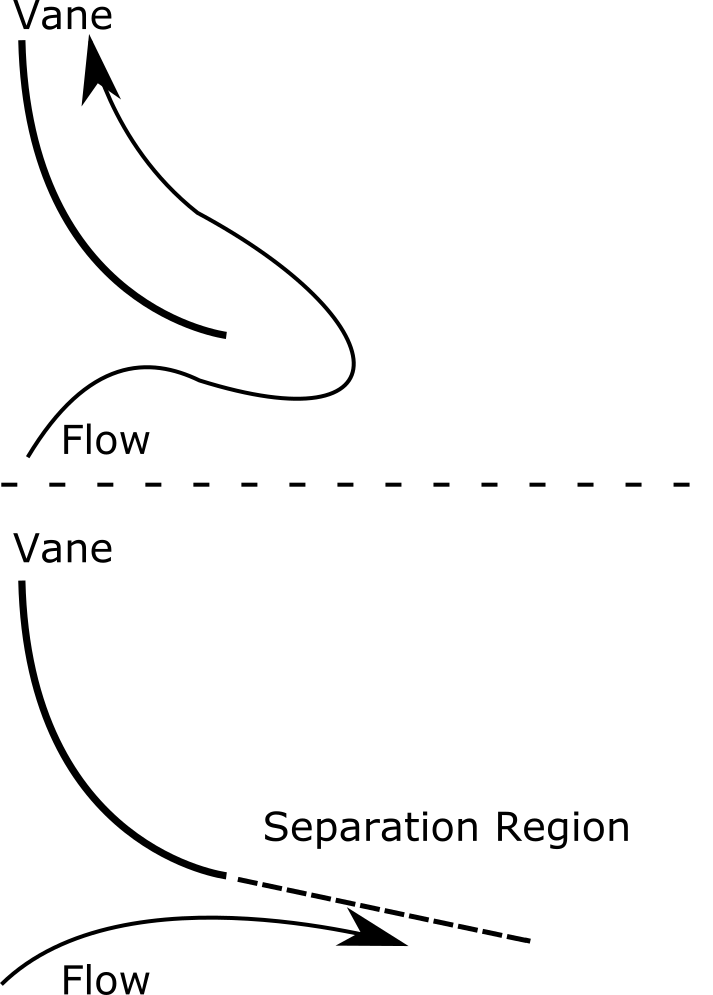
\includegraphics[width = 6 cm]{figs/sep_model}
    \caption{Schematic depicting the separation model that extends past the tailing edge of the vanes.}
    \label{fig:sep_model}
  \end{center}
\end{figure}

We have therefore introduced a simple separation model that modifies the forcing in use for an extended
region past the edges of the vanes. In the case where the flow is both leaving the vane region and 
the velocity vector of the fluid is pointing across the tangent line from the trailing edge of the vane edge, 
we force the flow as if the vane continued in a straight line past the trailing edge. This is designed to 
act as if there was a rigid surface past the vane edge, and gives the appearance of a special 
``no-penetration'' condition for the velocity for these cases. An image depicting these two cases in shown in 
figure \ref{fig:sep_model}. The addition of this simple separation model significantly reduced the flow that 
penetrated the vanes, and was consistent with the observations provided by our experimental colleagues. 

\subsection{Surface Roughness}

Finally, we also have need to invoke more abstract body forces. 
Our principle use case is model the surface roughness
impact, which is expected to be non-trivial\cite{oke1987boundary}. This
is more straight-forward than the previous cases, where the forcing is
simply defined uniformly over a region and set based on, 
\begin{equation}
 F = \frac{1}{2}\rho V^2 A_F. 
\end{equation}
The total energy injected into the flow can be measured as, 
\begin{equation}
 E_{\text{injected}} = \int_0^\infty F dz. 
\end{equation}
We ensure that the energy introduced into flow is small fraction of
total flow energy by comparing this with the energy flux through the top
of the vanes. 
This general forcing provides additional capabilities including the
ability to investigate engineering greater surface roughness or
structures that could provide greater ``kick-up'' of the thin thermal
layer near the surface into the flowing regime. It can also support more
general turning configurations than the virtual vanes outlined above. 
